\documentclass[pdf]{beamer}
\mode<presentation>{
	\usetheme{Ilmenau}
	
}
\usecolortheme{dolphin}
%\usepackage[UTF8,indent]{ctexcap}%中文
\usepackage{amssymb}
\usepackage{amsmath}
\usepackage{amsfonts}
%\usepackage{graphicx}
\usepackage{amsthm}
\usepackage{indentfirst}
\usepackage{enumerate}
\usepackage{extpfeil}
\usepackage{tikz-cd}
\usepackage{longtable}
\usepackage{makecell}
\usepackage{array}
\usepackage{xcolor}
\usetikzlibrary {calc,positioning,shapes.misc,graphs,decorations.pathreplacing}
\usepackage{hyperref}
\hypersetup{
colorlinks=true,
linkcolor=blue,
urlcolor=blue,
}
\usepackage{adjustbox}
\numberwithin{equation}{section}

\theoremstyle{plain}
\newtheorem{proposition}[theorem]{Proposition}
\newtheorem{claim}[theorem]{Claim}
\newtheorem{defn}[theorem]{Definition}
\newtheorem{eg}{  }
\newtheorem{pf}[theorem]{Proof}
\newtheorem{cor}[theorem]{Corollary}


\newtheorem{tabloid}[theorem]{Tabloid: equivalence class of standard filling}


\theoremstyle{plain}
\newtheorem{exercise}{Exercise}[section]


\theoremstyle{remark}
\newtheorem{remark}[theorem]{Remark}
\newtheorem{remarks}{Remarks}
\newtheorem{ex}[theorem]{Exercise}
\newtheorem{question}[theorem]{Questions}
\newtheorem{notation}[theorem]{Notations}
\newtheorem{short}{ }
\newtheorem{shortapp}[theorem]{Application}


\newcommand*{\thick}[1]{\text{\boldmath$#1$}}
\newcommand*{\cir}[1]{\;$\ding{19#1}$\;}%临时使用
\newcommand*{\norm}[1]{\lVert#1\rVert}
\newcommand*{\ignore}[1]{\textcolor{lightgray}{#1}}
\newcommand*{\stress}[1]{\textcolor{red}{#1}}
\newcommand*{\bgpicb}[1]{\usebackgroundtemplate{%
	\begin{tikzpicture}[path image/.style={
		path picture={
			\node at (path picture bounding box.center) {
				\includegraphics[height=10cm]{#1}
			};
	}}]
	
	\draw [path image]
	(current page.north west) rectangle
	(current page.south east);
	
	\end{tikzpicture}
}}
\newcommand*{\bgpica}[1]{\usebackgroundtemplate{%
		\begin{tikzpicture}[path image/.style={
			path picture={
				\node at (path picture bounding box.center) {
					\includegraphics[height=7.5cm]{#1}
				};
		}}]
		
		\draw [path image]
		(current page.north west) rectangle
		(current page.south east);
		
		\end{tikzpicture}
}}


\DeclareMathOperator{\supp}{supp}
\DeclareMathOperator{\dist}{dist}
\DeclareMathOperator{\vol}{vol}
\DeclareMathOperator{\diag}{diag}
\DeclareMathOperator{\tr}{tr}
\DeclareMathOperator{\Ker}{\operatorname{ker}}
\DeclareMathOperator{\coker}{\operatorname{coker}}
\DeclareMathOperator{\Proj}{\operatorname{Proj}}
\DeclareMathOperator{\Aut}{\operatorname{Aut}}
\DeclareMathOperator{\Img}{\operatorname{Im}}
\DeclareMathOperator{\Sym}{\operatorname{Sym}}
\DeclareMathOperator{\sgn}{\operatorname{sgn}}
\DeclareMathOperator{\Mod}{\operatorname{mod}}
\DeclareMathOperator{\Id}{\operatorname{Id}}
\DeclareMathOperator{\Hom}{\operatorname{Hom}}
\DeclareMathOperator{\Ext}{\operatorname{Ext}}
\DeclareMathOperator{\Tor}{\operatorname{Tor}}
\DeclareMathOperator{\rep}{\operatorname{rep}}
\DeclareMathOperator{\Irr}{\operatorname{Irr}}
\DeclareMathOperator{\ind}{\operatorname{ind}}
\DeclareMathOperator{\dvct}{\underline{\operatorname{dim}}}
\DeclareMathOperator{\ques}{\;?\;}
\DeclareMathOperator{\Fl}{\mathcal{F\ell}}
%\setlength{\parindent}{1em}




\setbeamertemplate{caption}[numbered]
% 设置图形文件的搜索路径
\graphicspath{{figures/}}
\title{Auslander--Reiten theory}
\author{Xiaoxiang Zhou}
\institute[Bonn uni]{Universität Bonn}
\date{\today} % March 24,2022
\tikzset{
	invisible/.style={opacity=0,text opacity=0},
	visible on/.style={alt=#1{}{invisible}},
	alt/.code args={<#1>#2#3}{%
		\alt<#1>{\pgfkeysalso{#2}}{\pgfkeysalso{#3}} % \pgfkeysalso doesn't change the path
	},
}
%\setbeamercolor{section number projected}{fg=white!90!blue, bg=red!90!black}
\definecolor{goodblue}{RGB}{71,71,186}
\definecolor{janblue}{RGB}{230, 230, 254}
\definecolor{jangreen}{RGB}{231, 255, 231}
\definecolor{olivegreen}{RGB}{60, 128, 49}


\setbeamercolor{block title}{fg=white, bg=goodblue}
\setbeamercolor{block body}{fg=black,bg=janblue}

\BeforeBeginEnvironment{defn}{
    \setbeamercolor{block title}{bg=olivegreen}
    \setbeamercolor{block body}{fg=black, bg=jangreen}
}
\AfterEndEnvironment{defn}{
 \setbeamercolor{block title}{fg=white, bg=goodblue}
 \setbeamercolor{block body}{fg=black,bg=janblue}
}
\BeforeBeginEnvironment{notation}{
    \setbeamercolor{block title}{bg=olivegreen}
    \setbeamercolor{block body}{fg=black, bg=jangreen}
}
\AfterEndEnvironment{notation}{
 \setbeamercolor{block title}{fg=white, bg=goodblue}
 \setbeamercolor{block body}{fg=black,bg=janblue}
}
\definecolor{ashgrey}{rgb}{0.7, 0.75, 0.71}
\usefonttheme[onlymath]{serif}
\usepackage[T1]{fontenc}
\usepackage{lmodern}

\setbeamertemplate{headline}{
	\begin{beamercolorbox}[wd=\paperwidth,ht=2.5ex,dp=1.125ex]{section in head/foot}%
		\hspace{3ex}{\insertsectionhead}
	\end{beamercolorbox}
	%	\begin{beamercolorbox}[ht=2.5ex,dp=1.125ex,leftskip=.3cm,rightskip=.3cm plus1fil]{subsection in head/foot}
	%		\usebeamerfont{subsection in head/foot}\insertsubsectionhead
	%\end{beamercolorbox}
}%删除点
\begin{document}
\begin{frame}
	\titlepage
	Jan Schröer's lecture notes should be a perfect reference. 
\end{frame}
\begin{frame}
In this talk, we dive into the huge forest of Auslander--Reiten theory.
\vspace{1cm}
\begin{table}[]
\begin{tabular}{c|c|c}
\hline
                 & Last time     & This time            \\ \hline
Central concepts & quiver rep    & ind rep \& AR quiver \\ \hline
Proofs           & relative easy & most skipped         \\ \hline
Goal             & comprehend    & enjoy                \\ \hline
\end{tabular}
\end{table}
\end{frame}

\begin{frame}{Review}
\begin{ex}
\centering
    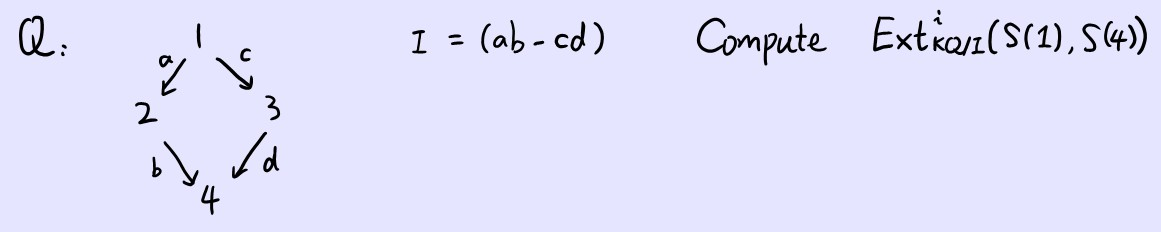
\includegraphics[scale=0.45]{figure/fig1.jpg}
    \vspace{2.5cm}
\end{ex}
\begin{defn}
$$\dvct M:= \left( \dim_K M_i \right)_{i \in v(Q)} \qquad \text{for } M \in \Mod(KQ/I)$$
\end{defn}
\end{frame}
%say something about "Later, we will represent representations by its dimension vector"
\begin{frame}[fragile]{Process}

\begin{itemize}
	\item Find more representations.
	\begin{itemize}
	\item knitting process
	\item introduction to root system
	\item relations among indecomposable representations\\
	(Compute $\Hom$, $\Ker$, $\coker$ in a fancy way) 
	\item starting function 
	\end{itemize}
	\vspace{0.5cm}
	\item From Dynkin quiver to affine quiver.
	\begin{itemize}
	\item knitting process
	\item new root system
	\item tube
	\item other cases
	\end{itemize}
\end{itemize}

\end{frame}

%Process:knitting

%在这个frame中adjustbox里面\textheight指的是页面上下之间的距离,\paperwidth是左右之间的距离,但要注意他们的长度都被scale了
\begin{frame}[fragile]{E.g. $A_5 \qquad 1 \stackrel{a}{\longrightarrow} 2 \stackrel{b}{\longrightarrow} 3 \stackrel{c}{\longleftarrow} 4
\stackrel{d}{\longrightarrow} 5 $}

\begin{overlayarea}{\linewidth}{\textheight}
\begin{short}
\adjustbox{minipage=[b][1\textheight][t]{2\paperwidth},scale=0.5,center}{%
% https://q.uiver.app/?q=WzAsNSxbMCwwLCIxIl0sWzEsMSwiMiJdLFsyLDIsIjMiXSxbMywxLCI0Il0sWzQsMiwiNSJdLFswLDFdLFsxLDJdLFszLDJdLFszLDRdXQ==
\[\begin{tikzcd}[column sep={2cm,between origins},row sep={6mm,between origins}]
	1 \\
	& 2 && 4 \\
	&& 3 && 5
	\arrow[from=1-1, to=2-2]
	\arrow[from=2-2, to=3-3]
	\arrow[from=2-4, to=3-3]
	\arrow[from=2-4, to=3-5]
\end{tikzcd}\]
\vspace{5mm}
% https://q.uiver.app/?q=WzAsNSxbMCwyLCJQKDEpIl0sWzEsMSwiUCgyKSJdLFsyLDAsIlAoMykiXSxbMywxLCJQKDQpIl0sWzQsMCwiUCg1KSJdLFsxLDBdLFsyLDFdLFsyLDNdLFs0LDNdXQ==
\[\begin{tikzcd}[column sep={2cm,between origins},row sep={13mm,between origins}]
	&& {P(3)} && {P(5)} \\
	& {P(2)} && {P(4)} \\
	{P(1)}
	\arrow[from=2-2, to=3-1]
	\arrow[from=1-3, to=2-2]
	\arrow[from=1-3, to=2-4]
	\arrow[from=1-5, to=2-4]
\end{tikzcd}\] 
}
\end{short}  
\begin{ex}
$a\colon i \rightarrow j \Longrightarrow f^a\colon P(j) \rightarrow P(i)$ is unique up to (nonzero) scalar.
\end{ex}
\end{overlayarea}
\end{frame}

\begin{frame}[fragile]{E.g. $A_5 \qquad 1 \stackrel{a}{\longrightarrow} 2 \stackrel{b}{\longrightarrow} 3 \stackrel{c}{\longleftarrow} 4
\stackrel{d}{\longrightarrow} 5 $}

\begin{overlayarea}{\linewidth}{\textheight}
\begin{short}
\adjustbox{minipage=[b][1.5\textheight][t]{2\paperwidth},scale=0.5,center}{%
% https://q.uiver.app/?q=WzAsNSxbMCwwLCIxIl0sWzEsMSwiMiJdLFsyLDIsIjMiXSxbMywxLCI0Il0sWzQsMiwiNSJdLFswLDFdLFsxLDJdLFszLDJdLFszLDRdXQ==
\[\begin{tikzcd}[column sep={2cm,between origins},row sep={6mm,between origins}]
	1 \\
	& 2 && 4 \\
	&& 3 && 5
	\arrow[from=1-1, to=2-2]
	\arrow[from=2-2, to=3-3]
	\arrow[from=2-4, to=3-3]
	\arrow[from=2-4, to=3-5]
\end{tikzcd}\]
\vspace{1mm}
%非常折磨人的微调。你知道为啥出现了偏差吗?效果是前后页面的箭头重叠。

% https://q.uiver.app/?q=WzAsNSxbMCwyLCIxMTEwMCJdLFsxLDEsIjAxMTAwIl0sWzIsMCwiMDAxMDAiXSxbMywxLCIwMDExMSJdLFs0LDAsIjAwMDAxIl0sWzEsMCwiZl5hIiwyXSxbMiwxLCJmXmIiLDJdLFsyLDMsImZeYyJdLFs0LDMsImZeZCIsMl1d
\[\begin{tikzcd}[column sep={2cm,between origins},row sep={13mm,between origins}]
	&& 00100 && 00001 \\
	& 01100 && 00111 \\
	11100
	\arrow["{f^a}"', from=2-2, to=3-1]
	\arrow["{f^b}"', from=1-3, to=2-2]
	\arrow["{f^c}", from=1-3, to=2-4]
	\arrow["{f^d}"', from=1-5, to=2-4]
\end{tikzcd}\]
}

\end{short}  

\end{overlayarea}
\end{frame}

\begin{frame}[fragile]{E.g. $A_5 \qquad 1 \stackrel{a}{\longrightarrow} 2 \stackrel{b}{\longrightarrow} 3 \stackrel{c}{\longleftarrow} 4
\stackrel{d}{\longrightarrow} 5 $}

\begin{overlayarea}{\linewidth}{\textheight}
\begin{short}
\adjustbox{minipage=[b][1\textheight][t]{2\paperwidth},scale=0.5,center}{%
% https://q.uiver.app/?q=WzAsNSxbMCwwLCIxIl0sWzEsMSwiMiJdLFsyLDIsIjMiXSxbMywxLCI0Il0sWzQsMiwiNSJdLFswLDFdLFsxLDJdLFszLDJdLFszLDRdXQ==
\[\begin{tikzcd}[column sep={2cm,between origins},row sep={6mm,between origins}]
	1 \\
	& 2 && 4 \\
	&& 3 && 5
	\arrow[from=1-1, to=2-2]
	\arrow[from=2-2, to=3-3]
	\arrow[from=2-4, to=3-3]
	\arrow[from=2-4, to=3-5]
\end{tikzcd}\]
\vspace{1mm}

% https://q.uiver.app/?q=WzAsNSxbMCwyLCIxMTEwMCJdLFsxLDEsIjAxMTAwIl0sWzIsMCwiMDAxMDAiXSxbMywxLCIwMDExMSJdLFs0LDAsIjAwMDAxIl0sWzEsMCwiZl5hIiwyXSxbMiwxLCJmXmIiLDJdLFsyLDMsImZeYyJdLFs0LDMsImZeZCIsMl1d
\[\begin{tikzcd}[column sep={2cm,between origins},row sep={13mm,between origins}]
	&& 00100 && 00001 \\
	& 01100 && 00111 \\
	11100
	\arrow["{f^a}"', from=2-2, to=3-1]
	\arrow["{f^b}"', from=1-3, to=2-2]
	\arrow["{f^c}", from=1-3, to=2-4]
	\arrow["{f^d}"', from=1-5, to=2-4]
\end{tikzcd}\]
}

\end{short}
\begin{short}[Initial case]
\begin{center}
\begin{tikzpicture}[baseline= (a).base]
\node[scale=0.5] (a) at (0,0){
% https://q.uiver.app/?q=WzAsMTAsWzAsMCwiMCJdLFsxLDAsIjAwMDAxIl0sWzIsMCwiMDAxMTEiXSxbMywwLCJcXGNva2VyIGZeZCJdLFs0LDAsIjAiXSxbNCwxLCIwIl0sWzAsMSwiMCJdLFsxLDEsIjAwMTAwIl0sWzIsMSwiMDExMDAgXFxvcGx1cyAwMDExMSJdLFszLDEsIlxcY29rZXIgXFxsZWZ0KFxcYmVnaW57c21hbGxtYXRyaXh9IGZeYlxcXFwgZl5jIFxcZW5ke3NtYWxsbWF0cml4fVxccmlnaHQpIl0sWzAsMV0sWzYsN10sWzcsOCwiXFxsZWZ0KFxcYmVnaW57c21hbGxtYXRyaXh9IGZeYlxcXFwgZl5jIFxcZW5ke3NtYWxsbWF0cml4fVxccmlnaHQpIl0sWzEsMiwiZl5kIl0sWzIsM10sWzgsOV0sWzksNV0sWzMsNF1d
\begin{tikzcd}[column sep={5mm},row sep={2mm}]
	0 & 00001 & 00111 & {\coker f^d} & 0 \\
	0 & 00100 & {01100 \oplus 00111} & {\coker \left(\begin{smallmatrix} f^b\\ f^c \end{smallmatrix}\right)} & 0
	\arrow[from=1-1, to=1-2]
	\arrow[from=2-1, to=2-2]
	\arrow["{\left(\begin{smallmatrix} f^b\\ f^c \end{smallmatrix}\right)}", from=2-2, to=2-3]
	\arrow["{f^d}", from=1-2, to=1-3]
	\arrow[from=1-3, to=1-4]
	\arrow[from=2-3, to=2-4]
	\arrow[from=2-4, to=2-5]
	\arrow[from=1-4, to=1-5]
\end{tikzcd}
};
\end{tikzpicture}
\end{center}
\end{short}
\end{overlayarea}
\end{frame}
%在这里可以看到可怕的套娃:frame+overlayarea是beamer的排版,short是其中一块,center居中,tikzpicture缩放,最后tikzcd是实际内容。我希望以后套娃能短点:<

\begin{frame}[fragile]{E.g. $A_5 \qquad 1 \stackrel{a}{\longrightarrow} 2 \stackrel{b}{\longrightarrow} 3 \stackrel{c}{\longleftarrow} 4
\stackrel{d}{\longrightarrow} 5 $}

\begin{overlayarea}{\linewidth}{\textheight}
\begin{short}
\adjustbox{minipage=[b][1.5\textheight][t]{2\paperwidth},scale=0.5,center}{%
% https://q.uiver.app/?q=WzAsNSxbMCwwLCIxIl0sWzEsMSwiMiJdLFsyLDIsIjMiXSxbMywxLCI0Il0sWzQsMiwiNSJdLFswLDFdLFsxLDJdLFszLDJdLFszLDRdXQ==
\[\begin{tikzcd}[column sep={2cm,between origins},row sep={6mm,between origins}]
	1 \\
	& 2 && 4 \\
	&& 3 && 5
	\arrow[from=1-1, to=2-2]
	\arrow[from=2-2, to=3-3]
	\arrow[from=2-4, to=3-3]
	\arrow[from=2-4, to=3-5]
\end{tikzcd}\]
\vspace{5mm}
% https://q.uiver.app/?q=WzAsNyxbMCwyLCIxMTEwMCJdLFsxLDEsIjAxMTAwIl0sWzIsMCwiMDAxMDAiXSxbMywxLCIwMDExMSJdLFs0LDAsIjAwMDAxIl0sWzIsMiwiMDExMTEiXSxbNCwyLCIwMDExMCJdLFsxLDAsImZeYSIsMl0sWzIsMSwiZl5iIiwyXSxbMiwzLCJmXmMiXSxbNCwzLCJmXmQiLDJdLFsxLDUsImdeYiJdLFszLDUsImdeYyJdLFszLDYsImdeZCJdXQ==
\[\begin{tikzcd}[column sep={2cm,between origins},row sep={13mm,between origins}]
	&& 00100 && 00001 \\
	& 01100 && 00111 \\
	11100 && 01111 && 00110
	\arrow["{f^a}"', from=2-2, to=3-1]
	\arrow["{f^b}"', from=1-3, to=2-2]
	\arrow["{f^c}", from=1-3, to=2-4]
	\arrow["{f^d}"', from=1-5, to=2-4]
	\arrow["{g^b}", from=2-2, to=3-3]
	\arrow["{g^c}", from=2-4, to=3-3]
	\arrow["{g^d}", from=2-4, to=3-5]
\end{tikzcd}\]
}

\end{short}
  

\end{overlayarea}
\end{frame}

\begin{frame}[fragile]{E.g. $A_5 \qquad 1 \stackrel{a}{\longrightarrow} 2 \stackrel{b}{\longrightarrow} 3 \stackrel{c}{\longleftarrow} 4
\stackrel{d}{\longrightarrow} 5 $}

\begin{overlayarea}{\linewidth}{\textheight}
\begin{short}
\adjustbox{minipage=[b][1.3\textheight][t]{2\paperwidth},scale=0.5,center}{%
% https://q.uiver.app/?q=WzAsNSxbMCwwLCIxIl0sWzEsMSwiMiJdLFsyLDIsIjMiXSxbMywxLCI0Il0sWzQsMiwiNSJdLFswLDFdLFsxLDJdLFszLDJdLFszLDRdXQ==
\[\begin{tikzcd}[column sep={2cm,between origins},row sep={6mm,between origins}]
	1 \\
	& 2 && 4 \\
	&& 3 && 5
	\arrow[from=1-1, to=2-2]
	\arrow[from=2-2, to=3-3]
	\arrow[from=2-4, to=3-3]
	\arrow[from=2-4, to=3-5]
\end{tikzcd}\]
\vspace{5mm}
% https://q.uiver.app/?q=WzAsMTUsWzAsMiwiMTExMDAiXSxbMSwxLCIwMTEwMCJdLFsyLDAsIjAwMTAwIl0sWzMsMSwiMDAxMTEiXSxbNCwwLCIwMDAwMSJdLFsyLDIsIjAxMTExIl0sWzQsMiwiMDAxMTAiXSxbMSwzLCIxMTExMSJdLFswLDQsIjAwMDExIl0sWzEsNSwiMDAwMTAiXSxbMiw0LCIxMTExMCJdLFszLDMsIjAxMTEwIl0sWzMsNSwiMTEwMDAiXSxbNCw2LCIxMDAwMCJdLFs0LDQsIjAxMDAwIl0sWzEsMF0sWzIsMV0sWzIsM10sWzQsM10sWzEsNV0sWzMsNV0sWzMsNl0sWzAsN10sWzcsOF0sWzgsOV0sWzUsN10sWzcsMTBdLFsxMCw5XSxbNSwxMV0sWzYsMTFdLFsxMSwxMF0sWzEwLDEyXSxbMTIsMTNdLFsxMSwxNF0sWzE0LDEyXV0=
\[\begin{tikzcd}[column sep={2cm,between origins},row sep={13mm,between origins}]
	&& 00100 && 00001 \\
	& 01100 && 00111 \\
	11100 && 01111 && 00110 \\
	& 11111 && 01110 \\
	00011 && 11110 && 01000 \\
	& 00010 && 11000 \\
	&&&& 10000
	\arrow[from=2-2, to=3-1]
	\arrow[from=1-3, to=2-2]
	\arrow[from=1-3, to=2-4]
	\arrow[from=1-5, to=2-4]
	\arrow[from=2-2, to=3-3]
	\arrow[from=2-4, to=3-3]
	\arrow[from=2-4, to=3-5]
	\arrow[from=3-1, to=4-2]
	\arrow[from=4-2, to=5-1]
	\arrow[from=5-1, to=6-2]
	\arrow[from=3-3, to=4-2]
	\arrow[from=4-2, to=5-3]
	\arrow[from=5-3, to=6-2]
	\arrow[from=3-3, to=4-4]
	\arrow[from=3-5, to=4-4]
	\arrow[from=4-4, to=5-3]
	\arrow[from=5-3, to=6-4]
	\arrow[from=6-4, to=7-5]
	\arrow[from=4-4, to=5-5]
	\arrow[from=5-5, to=6-4]
\end{tikzcd}\]
}
The constructed quiver is called the \textbf{Auslander--Reiten quiver}, and the process is called the \textbf{knitting algorithm}.
\end{short}
  

\end{overlayarea}
\end{frame}
%参考:https://tex.stackexchange.com/questions/254285/increasing-the-text-size-of-tikz-cd-labels
\begin{frame}[fragile]{Another example: $D_4 \qquad$% https://q.uiver.app/?q=WzAsNCxbMCwxLCIxIl0sWzEsMSwiMiJdLFsyLDEsIjMiXSxbMSwwLCI0Il0sWzAsMV0sWzIsMV0sWzMsMV1d
\begin{tikzcd}[sep={3mm},font = \small, ampersand replacement=\&]
	\& 4 \\
	1 \& 2 \& 3
	\arrow[from=2-1, to=2-2]
	\arrow[from=2-3, to=2-2]
	\arrow[from=1-2, to=2-2]
\end{tikzcd}}

\begin{overlayarea}{\linewidth}{\textheight}
\begin{short}
\adjustbox{minipage=[b][1.3\textheight][t]{2\paperwidth},scale=0.5,center}{%
% https://q.uiver.app/?q=WzAsNCxbMCwwLCIxIl0sWzEsMSwiMiJdLFsyLDAsIjMiXSxbMywwLCI0Il0sWzAsMV0sWzIsMV0sWzMsMV1d
\[\begin{tikzcd}[column sep={2cm,between origins},row sep={8mm,between origins}]
	1 &&[-15mm] 3 & 4 \\
	& 2
	\arrow[from=1-1, to=2-2]
	\arrow[from=1-3, to=2-2]
	\arrow[from=1-4, to=2-2]
\end{tikzcd}\]

\vspace{5mm}
% https://q.uiver.app/?q=WzAsMTIsWzEsMCwiXFxzdWJzdGFja3swXFxcXDAxMH0iXSxbMCwxLCJcXHN1YnN0YWNrezBcXFxcMTEwfSJdLFsyLDEsIlxcc3Vic3RhY2t7MFxcXFwwMTF9Il0sWzMsMSwiXFxzdWJzdGFja3sxXFxcXDAxMH0iXSxbMSwyLCJcXHN1YnN0YWNrezFcXFxcMTIxfSJdLFswLDMsIlxcc3Vic3RhY2t7MVxcXFwwMTF9Il0sWzIsMywiXFxzdWJzdGFja3sxXFxcXDExMH0iXSxbMywzLCJcXHN1YnN0YWNrezBcXFxcMTExfSJdLFswLDUsIlxcc3Vic3RhY2t7MFxcXFwxMDB9Il0sWzIsNSwiXFxzdWJzdGFja3swXFxcXDAwMX0iXSxbMyw1LCJcXHN1YnN0YWNrezFcXFxcMDAwfSJdLFsxLDQsIlxcc3Vic3RhY2t7MVxcXFwxMTF9Il0sWzAsMV0sWzAsMl0sWzAsM10sWzEsNF0sWzIsNF0sWzMsNF0sWzQsNV0sWzQsNl0sWzQsN10sWzUsMTFdLFs2LDExXSxbNywxMV0sWzExLDhdLFsxMSw5XSxbMTEsMTBdXQ==
\[\begin{tikzcd}[column sep={2cm,between origins},row sep={13mm,between origins}]
	& {\substack{0\\010}}&[-15mm]& \\
	{\substack{0\\110}} && {\substack{0\\011}} & {\substack{1\\010}} \\
	& {\substack{1\\121}} \\
	{\substack{1\\011}} && {\substack{1\\110}} & {\substack{0\\111}} \\
	& {\substack{1\\111}} \\
	{\substack{0\\100}} && {\substack{0\\001}} & {\substack{1\\000}}
	\arrow[from=1-2, to=2-1]
	\arrow[from=1-2, to=2-3]
	\arrow[from=1-2, to=2-4]
	\arrow[from=2-1, to=3-2]
	\arrow[from=2-3, to=3-2]
	\arrow[from=2-4, to=3-2]
	\arrow[from=3-2, to=4-1]
	\arrow[from=3-2, to=4-3]
	\arrow[from=3-2, to=4-4]
	\arrow[from=4-1, to=5-2]
	\arrow[from=4-3, to=5-2]
	\arrow[from=4-4, to=5-2]
	\arrow[from=5-2, to=6-1]
	\arrow[from=5-2, to=6-3]
	\arrow[from=5-2, to=6-4]
\end{tikzcd}\]
}
For other examples, see \href{https://github.com/ramified/personal_handwritten_collection/raw/c5f6429469b144c8ba72a0ca41f45d70ff8a2709/weeklyupdate/2021.08.15_indec_rep_of_Dynkinquiver.pdf}{here}.
\end{short}
  

\end{overlayarea}
\end{frame}
\begin{frame}[fragile]{Questions}

\begin{itemize}
	\item How many indecomposable representations are there?
	\item Do those dimension vectors follow any patterns?
	\item Where are those irreducible/projective/injective representations?
\end{itemize}

\end{frame}

%Process:root system


\end{document}
%Process: red and gray


%\begin{equation*}
%\begin{aligned}
%内容...
%\end{aligned}
%\end{equation*}
